% include the figures path relative to the master file
\graphicspath{ {./content/intro/figures/} }

\section{Introduction}
\label{sec:descr}  % \label{} allows reference to this section
Despite the fact that malignant melanoma only accounts for nearly 2\% of all skin cancer cases, the vast majority of skin cancer deaths are due to malignant melanoma.
According to the World Health Organisation, during the past decades, the incidence of this pathology has increased up to $132,000$ diagnosed cases of melanoma~\cite{WoH}.
The \Ac{acs} estimated that during 2014 there would be diagnosed $76,100$ new cases of melanoma, leading to death in $9710$ cases  ~\cite{CancerFactsFigures2014}.
At advanced stage, melanoma is incurable and the patients should go through surgery, possibly immunotherapy, chemotherapy, and/or radiation therapy.
However, if diagnosed at its early stage, melanoma is the most treatable kind of cancer~\cite{CancerFactsFigures2014,forsea2012melanoma}.

Due to this tractability of early detected melanoma, and the efforts done during the last decades to develop methods to detect melanoma at this early stage, the patients' survival rate has well increased.
Among these methods, systematic screening and consistent criteria for visual inspection of skin lesions' images, acquired through different imaging techniques (\emph{i.e.}\,dermoscopy).
A well established criteria for early stage melanoma prognosis is the ``ABCDE'' rule~\cite{abbasi2004early} illustrated in \cref{fig:lexicon}.
This criteria is meant for a human reader to visually inspect an image of a skin lesion, and characterize this lesion based on the following visual cues:
\begin{enumerate}[label=(\Alph*)]
\item {\textbf A}symetry of the lesion
\item irregularity of the lesion {\textbf B}orders
\item presence of variegated {\textbf C}olors within the lesion
\item lesion size, evaluating if the {\textbf D}iameter of the lesion is greater than \SI{6}{\milli \meter}
\item evaluation of the lesion {\textbf E}volution over time, through regular screening.
\end{enumerate}

\begin{figure*}
\begin{center}
  \hspace*{\fill}
    \subfloat[melanoma]{
    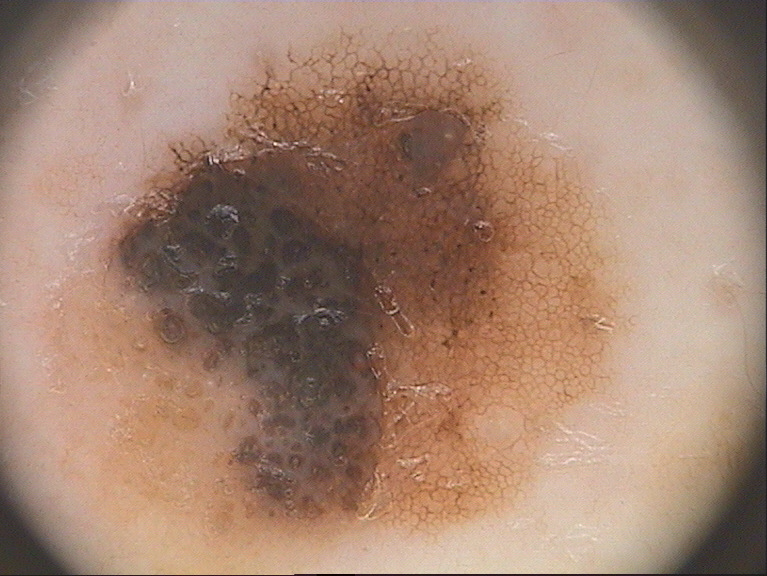
\includegraphics[width=0.19\textwidth,]{lexicon/melanoma_IMD406.png}}\hfill
    \subfloat[{\textbf A}ssimetric]{
    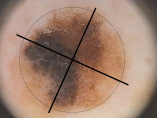
\includegraphics[width=0.19\textwidth,]{lexicon/melanoma_A.png}}\hfill
    \subfloat[irregular {\textbf B}orders]{
    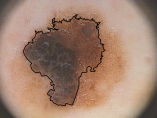
\includegraphics[width=0.19\textwidth,]{lexicon/melanoma_B.png}}\hfill
    \subfloat[variated {\textbf C}olors]{
    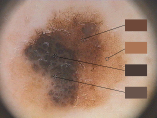
\includegraphics[width=0.19\textwidth,]{lexicon/melanoma_C.png}}\hfill
    \subfloat[{\textbf D}iameter]{
    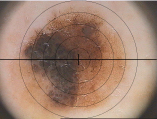
\includegraphics[width=0.19\textwidth,]{lexicon/melanoma_D.png}}\hfill
  \hspace*{\fill}
  \\
  \hspace*{\fill}
    \subfloat[benign lesion]{
    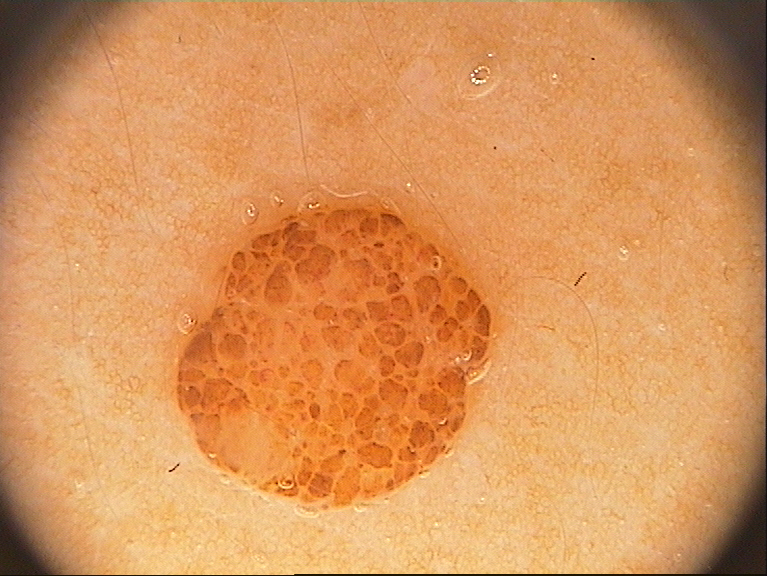
\includegraphics[width=0.19\textwidth,]{lexicon/IMD199.png}}\hfill
    \subfloat[non-{\textbf A}ssimetric]{
    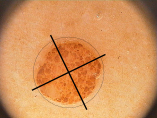
\includegraphics[width=0.19\textwidth,]{lexicon/good_A.png}}\hfill
    \subfloat[regular {\textbf B}orders]{
    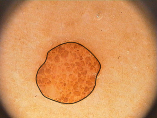
\includegraphics[width=0.19\textwidth,]{lexicon/good_B.png}}\hfill
    \subfloat[unique {\textbf C}olor]{
    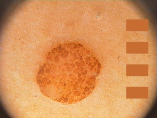
\includegraphics[width=0.19\textwidth,]{lexicon/good_C.png}}\hfill
    \subfloat[{\textbf D}iameter]{
    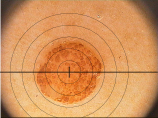
\includegraphics[width=0.19\textwidth,]{lexicon/good_D.png}}\hfill
  \hspace*{\fill}\\
    \caption{{\textbf ABCD}-lexicon comparison of two lesions. The top row corresponds to melanoma while the bottom row is a benign lesion.}
  \label{fig:lexicon}
\end{center}
\end{figure*}

Despite the aforesaid positive impact of these methodologies, visual inspection of medical images for diagnosis is prone to errors.
Manning\,\emph{et\,al.} state that the diagnosis error rates are comparable to the error rates found in any other human visual inspection task ~\cite{manning2014perception}.
Thus, double readings and \cad systems are placed to aid dermatologists and clinicians to mitigate this weakness.
A variety of the proposed \cad systems that take advantage of image processing and \ml to mimic the criteria defined by the ``ABCDE'' rule~\cite{rastgoo2015automatic}.
A prevalent schema for such \cad systems, consists of: image pre-processing to facilitate any subsequent task; segmentation to determine the extension of the lesion (emulating the reading of the image by a human grader); feature extraction to characterize the lesion; and further, classification of these features to drive the decision.
To describe the lesions using highly cognitive terms such as lesion asymmetry or boundary regularity, requires accurate delineation of the lesions. For the clinicians case, finding this delineation is intrinsic to the visual inspection. However, for the case of \cad systems, the delineation is subject to the process of segmentation, which remains an open research topic~\cite{duncan2000medical}.

In this paper, we propose a more general framework which does not need pre-processing and segmentation of the lesions.
The method exploits low-level features underling the visual process of segmentation, but instead of producing a segmentation these features are directly encoded as high-level features based on sparse coding to feed a \ac{rf} classifier~\cite{breiman2001random} to detect melanoma in dermoscopic images.  

The rest of this paper is organized as follows: an overview of related work is presented in Sect.\,\ref{sec:RW}.
The proposed method is discuss in Sect.\,\ref{sec:method} while the validation and obtained results are presented in Sect.\,\ref{sec:RE}.
Finally the paper is concluded in Sect.\,\ref{sec:conclusion}.

% \begin{figure*}
% \begin{center}
%   \hspace*{\fill}
%   \subfloat[Melanoma lesion]{
%     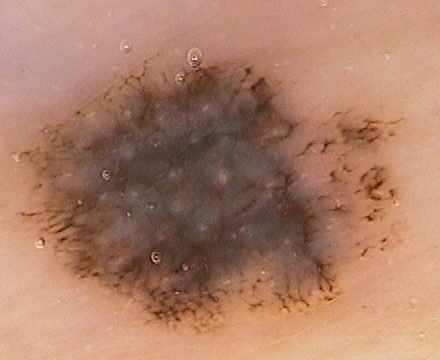
\includegraphics[width=0.2\textwidth, height= 0.12\textheight]{M1_PH2.png}}\hfill
%   \subfloat[Dysplastic lesion]{
%     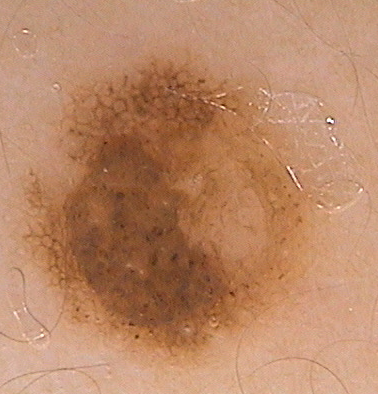
\includegraphics[width=0.2\textwidth, height= 0.12\textheight]{D1_PH2.png}}\hfill
%   \subfloat[Benign lesion]{
%     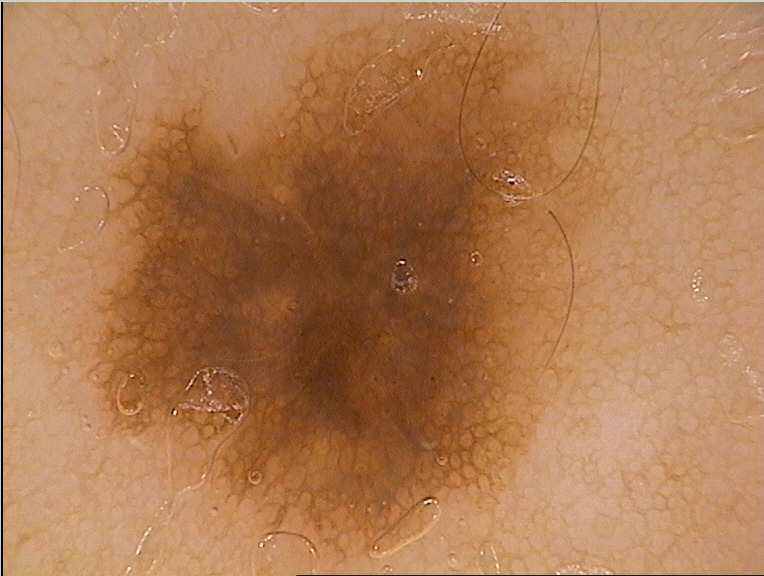
\includegraphics[width=0.2\textwidth, height= 0.12\textheight]{B1_PH2.png}}
%   \hspace*{\fill}
%   \caption{Samples of $PH^2$ dataset, representing melanoma, dysplastic and benign lesions, respectively.}
%   \label{fig:PH2samples}
% \end{center}
% \end{figure*}




% Some stuff that emac's colegues use
%%% Local Variables:
%%% mode: late
%%% TeX-master: "../../master.tex"
%%% End: \section{introduction}

